\documentclass[letterpaper, 10pt, conference]{ieeeconf}

\IEEEoverridecommandlockouts    % If we want to use the thanks command

\usepackage{fullpage}
\usepackage{color}
\usepackage{graphicx}
\usepackage{amsmath}
\usepackage{amssymb}
\usepackage{url}
\usepackage{subfig}
\usepackage{algorithmic}
\usepackage{algorithm}

% EPS2PDF stuff?

\newcommand{\xxx}[1]{\textcolor{red}{#1}}

\title{\LARGE \bf
    3D Environment Reconstruction Using RGB-D Visual Odometry
}

\author{Pedro d'Aquino, Paridhi Desai and John Peterson\thanks{Robert Goeddel and Lauren Hinkle
wrote parts of this report, as explained in the end of the document.}}


\begin{document}

\maketitle
%\thispagestyle{empty} % XXX These were in the IROS example, but I didn't read
                      % far enough along to see if they disappear later
%\pagestyle{empty}

\begin{abstract}
The reconstruction of environments in 3D can be challenging with just range
data. RGB-D sensors like the Microsoft Kinect provide visual details that
allow odometry to be used even in environments with ambiguous depth data.
This paper demonstrates a simplified implementation of Henry et al.'s work
on RGB-D Mapping.~\cite{Henry2010RGBd}
Our system can construct reasonably accurate models of
small to medium sized indoor environments in real time at resolutions of up
to 2\,cm and in near-real time at 1\,cm. By using SURF features from the image
data in conjunction with the Kinect's depth data, we are able to compute
accurate alignments of point clouds over time. Our system does not attempt to
implement the loop-closing portion of Henry et al.'s work.
\end{abstract}

\section{Introduction}
This paper will present a system capable of building detailed colored point
clouds using a consumer grade RGB-D sensor, the Microsoft Kinect. The
convenient availability of such sensors makes them an appealing budget option
for a small robot operating in an indoor environment where the limited range
of the Kinect is less of a concern. Furthermore, the colored point data
generated by RGB-D sensors can provide more robust alignments than even high
quality pure-range sensors such as LIDAR in environments with range-detectable
features.

LIDAR and other range based sensors may be used to generate extremely detailed
and accurate 3D point clouds that may be merged over time to reconstruct a 3D
model of an environment. Generally, these alignments are straightforward to
detect and such systems are fairly robust. However, there are some weaknesses.
A classic example is the so-called ``hallway problem.'' A common concern for
SLAM systems is that all stretches of a long hallway look the same. The lack
of distinguishing features mean that, while we may correctly align the walls
to run parallel to previously observed walls, it is difficult if not
impossible to constrain an observation to one particular location. Depending
on the reliability of a robot's odometry, this may cause compression or
expansion of the hallway in question. Features from associated image data can
make an otherwise indistinguishable segment of wall easy to align with
previous scans, as seen in Fig.~\ref{fig:cse-wall}.

The output of an RGB-D sensor can also be used for general 3D modeling
applications. Artists may spend days creating detailed models of objects from
the real world. Given an RGB-D sensor and a system capable of merging many
observations, an untrained user can wave the sensor around the object needing
to be modeled and automatically generate a 3D model complete with texture.
This preservation of visual data even aids in the end product of the mapping
task. Imagine a 3D map of a building created from range data. While the map
might be an accurate layout of the building, the lack of visual cues may still
leave the user feeling lost and confused while navigating through a virtual
reconstruction of this environment. Associated color data could
have features such as door numbers and maps of the building available to aid
in navigation.

\begin{figure}[t]
\centering
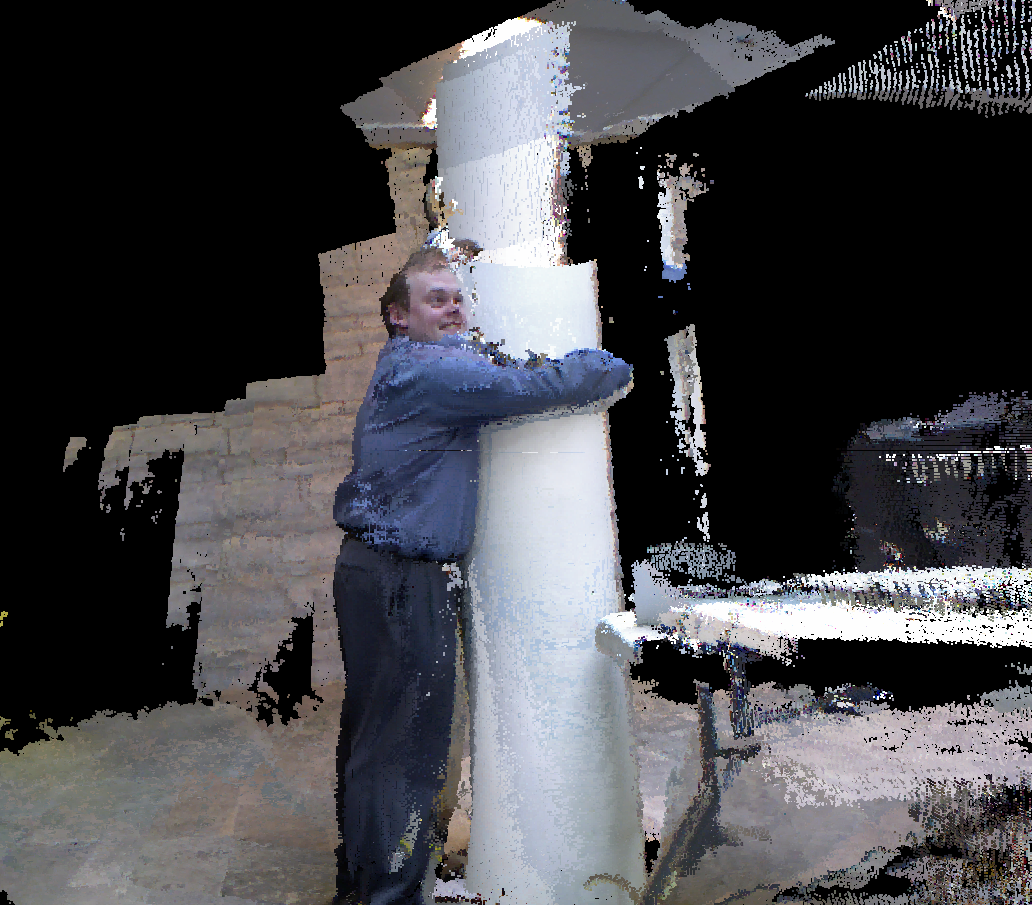
\includegraphics[width=0.48\textwidth]{figures/cropped_ed.png}
\caption{A model of Prof. Ed Olson.
Voxel resolution for this model is 0.5\,cm, allowing us to preserve details
such as the creases in Ed's shirt and pants or the pupils of his eyes.}
\label{fig:ed-model}
\end{figure}

% Figure spanning columns. Top of second page, probably
\begin{figure*}[t]
\centering
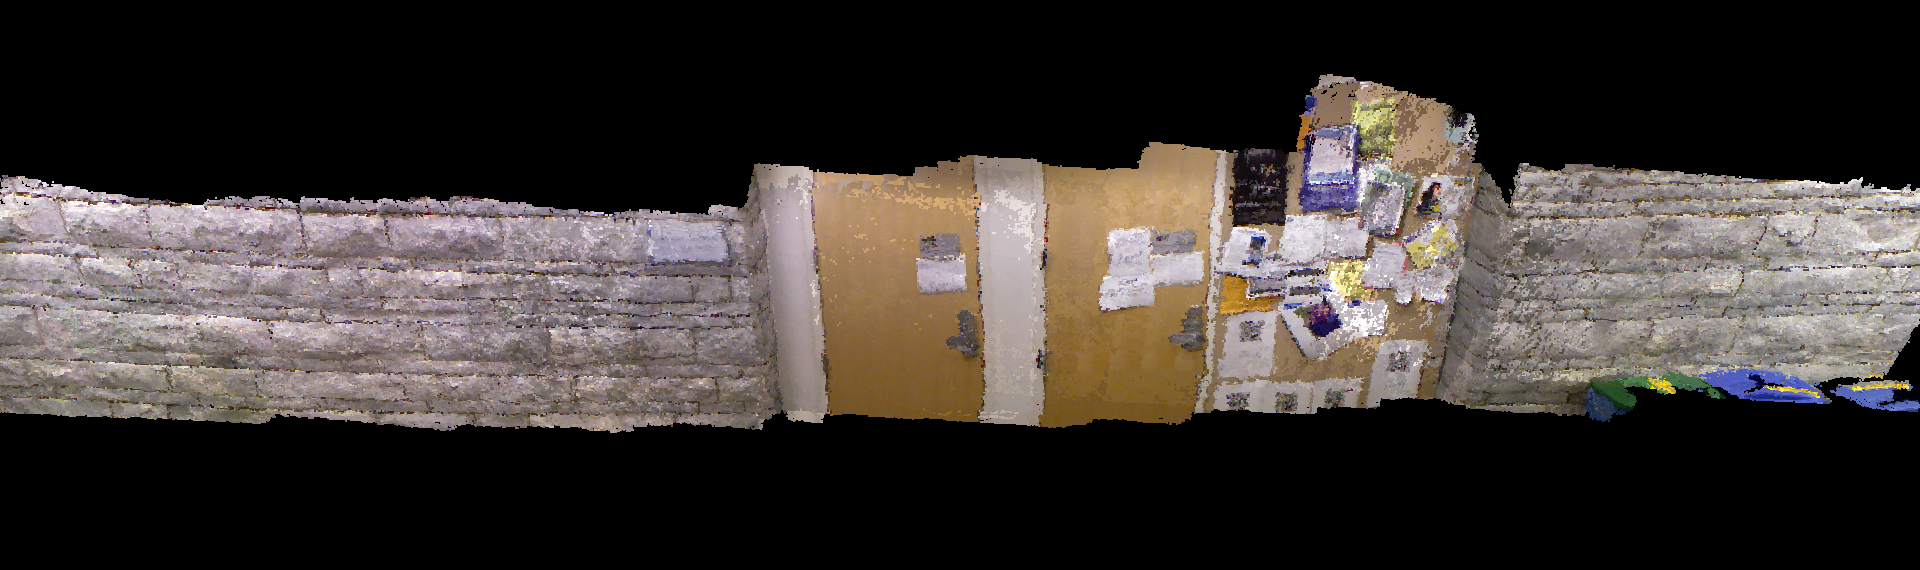
\includegraphics[width=.9\textwidth]{figures/CSE_Wall.png}
\caption{By using image features such as the corners of rocks in a wall,
combined color and depth data can be accurately placed into a global map even
in flat hallway situations. As seen above, even when depth features such as
the doorways and recycling bins go out of view, our system continues to build
an accurate model of the wall to the left of the doors.}
\label{fig:cse-wall}
\end{figure*}

\section{Previous Work}
Our work is a simplified reimplementation of the work of Peter Henry et
al~\cite{Henry2010RGBd}. Their work demonstrated a system capable of RGB-D
mapping using a conjunction of 3D SIFT alignment, plane-fitting ICP, and the
SLAM system TORO. By using visual features projected into 3D space to gain an
initial alignment between frames and by using ICP to converge the rest of the
way, Henry et al. were able to make a ``near-real time'' system capable of
producing very detailed 3D reconstructions. By maintaining periodic keyframes
for different locations, they are able to make large-scale loop closures by
recognizing those same features later, resulting in a very robust system.

To show their results, Henry et al. created what they call \emph{surfels}.
Surfels allow them to deal with the massive amounts of data provided by their
RGB-D sensor without losing significant detail about the scene. As videos of
their results demonstrate, the system is capable of preserving details such as
the pattern on carpet or slightly blurry versions of people's faces in
pictures.

Albert Huang and his group at MIT, working in conjunction with Henry et al. at
the University of Washington, were able to take this system a step further,
creating a real-time mapping system that allowed a quadrotor to autonomously
fly through cluttered 3D environments using a Kinect~\cite{Huang2011isrr}.
Huang et al.'s work adds data from IMUs and switches to FAST features to
support real time voxel mapping at a coarse resolution sufficient for
trajectory planning.

Recently, Pandey et al. worked on extending ICP using visual features~\cite{silviogicp}.
Their work focuses on laser scanner data, but bears resamblance to Henry et al.'s
RGBD-ICP.

\subsection{Contributions}
For this project, we have implemented a subset of the work of Henry et al.
Our implementation of RGB-D mapping passes entirely on the SLAM portion,
focusing instead on feature-based odometry. Lacking time to implement a
full RGB-D SLAM system capable of rendering real-time navigable scenes at the
level of detail demonstrated by Henry et al., we focused on making our system
real-time. This can be used to justify many of deviations from the original
implementation.

\section{Methodology}
Fig.~\ref{fig:blockdiagram} shows a block diagram of our system. The goal of the system is
to use RGB and depth image from the current and previous frames to find the rigid body transformation that moved
the camera between these frames, and then use this RBT to create a 3D map.

Firstly, SURF features are extracted from the RGB images, and combined with depth information to form 3D features.
These features are matched based on the euclidian distance among their descriptors.
The matches are refined using RANSAC, which also computes the optimal alignment between the inlier 3D feature pairs. This
initial estimate of the RBT is fed into RGBD-ICP, which tries to find the best alignment between the point clouds from
the two frames. The resulting alignment is the system's best guess of the RBT that moved the Kinect between the
two frames, and is used to project the color point cloud from the last frame into the 3D map.

\subsection{Kinect Data Acquisition and Calibration}

We used the open source OpenKinect C library, more commonly known as Libfreenect ~\cite{OpenKinect}, to acquire RGB images from the Kinects Color camera at a resolution of 640x480 pixels and to acquire the depth image of the scene that the Kinect computes also at a resolution of 640x480, though the block matching employed to compute the depth values means that the depth image only has an effective resolution of 632x480. An example of the data returned by the Kinect can be seen in Fig. \ref{fig:Kinect-demo}.

The Kinect generates this ``depth image''� by effectively solving the stereo camera problem in hardware and then outputting a value for each pixel that can be mapped to a depth value.  The Kinect uses an Infra-Red projector to shine a structured pattern onto the scene.  The Kinect also has an infrared camera which it uses to observe the pattern projected on the scene.  Together the projector and camera form a stereo pair allowing the Kinect to compute disparities and from that depth.  Through calibration at the manufacturer, the Kinect computes a disparity between a reference image of the IR pattern, effectively the view from the projector, and uses a 9x9 block matching algorithm to compute the disparity between this reference image and the actual pattern which is deformed by objects in the world.  The depth image is not actually in terms of meters but instead is in integers from 0 to 2047.  Using a depth model provided by Dr. Stephane Magnenat on the Open Kinect Website~\cite{OpenKinect}, we can convert these integers into a real depth value.  

This active lighting system for determining depth has several implications for the performance of the Kinect.  The limited power of the Kinect's projector limits the maximum range that it can measure to approximately 8 meters.  Furthermore accuracy rapidly falls off after 4 meters so we simply threw out points beyond this distance.   The Kinect is also subject to interference from other strong sources of IR light like the Sun, making it unsuitable for out door use.  There also may be the possibility for multiple Kinects to interfere with one another but we did not investigate this possibility since we were only considering a single Kinect rig.  

\begin{figure}
\centering
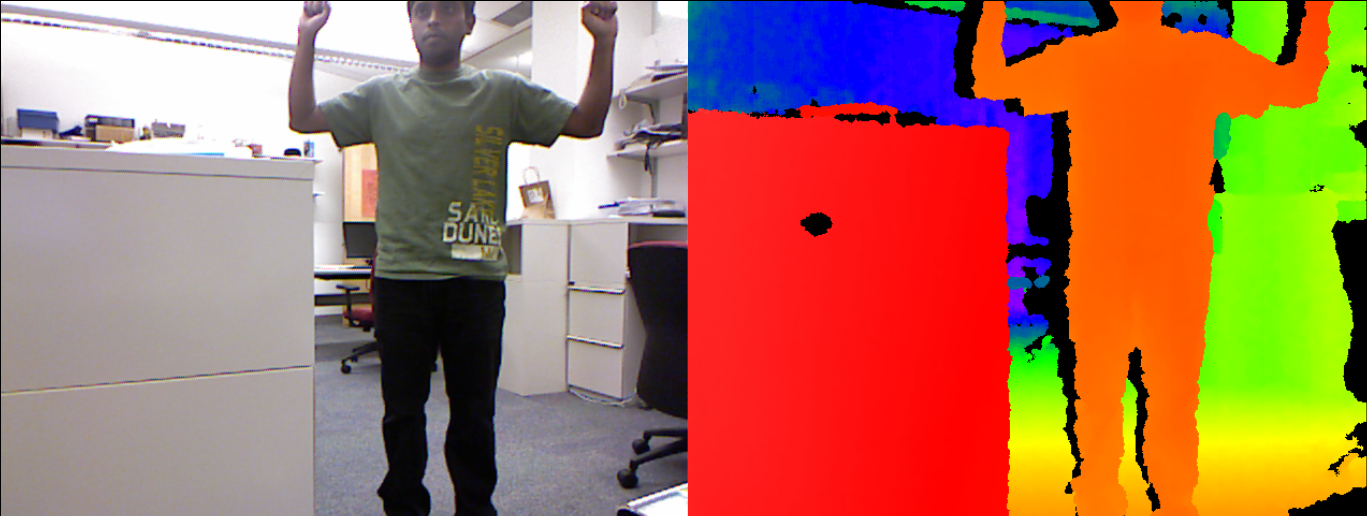
\includegraphics[width=0.48\textwidth]{figures/KinectDemo.png}
\caption{RGB and depth data from a Kinect. For easier consumption, the depth
data has been mapped through the colors of the rainbow where red corresponds
to objects roughly 1\,m away and purple corresponds to objects roughly 8~\,m
away. Though the maximum range is at least 8\,m, the depth data
becomes increasingly noisy, so we only use data within 3.8\,m of the Kinect,
the range at which the data seems to begin to deteriorate.}
\label{fig:Kinect-demo}
\end{figure}

Using this pair of color images of the scene, the depth image, and another stereo calibration, it is possible to generate a colored point cloud, a set of points in 3D relative to the Kinect with color values.  In the traditional stereo problem, the intrinsic parameters of each camera turn each pixel into rays out into the scene, which are epipolar lines when seen from the other camera.  However the Kinect makes this problem much easier because we have depth values for each of the pixels from the depth image's perspective.  This depth value means that rather than having a ray from the camera, we simply have a point in 3D space.  Then using the intrinsic parameters of the RGB camera combined with the rotation transformation relating the two frames it is easy to project this 3D point into pixel coordinates of the color image to get the point's color.  We repeat this process for each point in the depth image to generate a colored point cloud in the Kinect's local frame.  



\begin{figure*}[t]
\centering
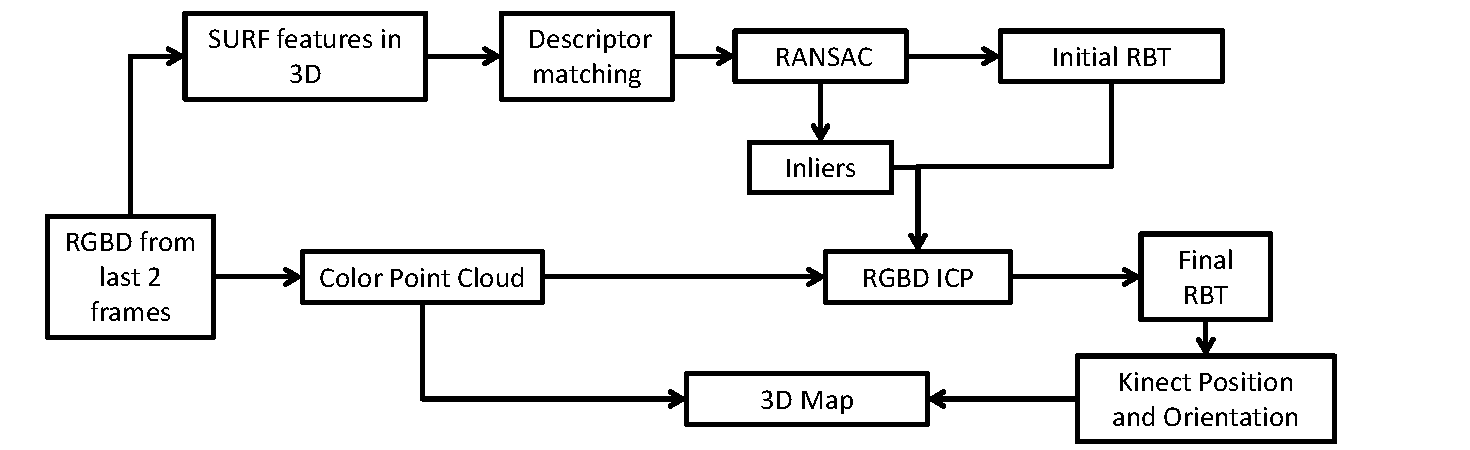
\includegraphics[width=1.0\textwidth]{figures/blockdiagram.pdf}
\caption{A block diagram of our proposed system.}
\label{fig:blockdiagram}
\end{figure*}

The above process requires an accurate estimate of the intrinsic parameters of both the RGB and IR cameras.  We initially used the Camera Calibration Toolbox for Matlab~\cite{MatlabCalibration} to extract the intrinsic camera parameters for each of the cameras.  These parameters include focal lengths optical axis and radial and tangential distortion parameters for Brown's distortion model.  Despite getting errors on the order of .5 pixel the parameters did not seem to yield a good result.  We calibrated our Kinect using Nicolas Burrus's RGBDemo toolkit ~\cite{BurrusCalibration}.  This software, like the Matlab Toolbox, also uses multiple images of a calibration target with both the IR and RGB cameras but also automatically handles the stereo calibration.  This calibration seemed to yield the best results out of several calibration attempts.  

Unfortunately this method is not quite perfect, perhaps due to an imperfect estimation of the camera parameters.  Get poor color estimates around edges in some cases, where colors in the background would appear on foreground objects and vice versa.  This error is visible in Fig.~\ref{fig:ed-model} where color from pole appears at the depth of his sleeve.  Overall accuracy seems sufficient to generate high quality point clouds that represent the environment that the Kinect sees but there is still room for improvement in this area. 

\subsection{Frame Matching Using Image Features}
The first approximation of the movement of the Kinect comes from matching 3D image
features between the current and the last frame. In this section, we describe the details
of our implementation.

\subsubsection{Feature Extraction and Description}
We compute SURF features and descriptors
to extract and describe features in the image~\cite{Bay06surf}. Our approach differs
from Henry et al., who use a parallel implementation of SIFT descriptors~\cite{SIFTGPU}.
As the majority of the development laptops we used had integrated graphics cards, using
a GPU implementation was not feasible. We found that SURF was an adequate tradeoff
between robustness and performance. Our implementation uses OpenCV~\cite{opencv_library}
for feature detection and descriptor extraction, with a JNI wrapper to allow for
communication with the rest of the system.

\subsubsection{Feature Matching}
We match a SURF feature to its nearest Euclidian neighbor in the other frame in the space
of SURF descriptors. The matching
uses a KD-tree for efficiency. We experimented with reducing the number of outliers by
constraining the matches in two ways. In the ``distant second'' approach, let $A_i$ be the
best match for feature $B_j$, with distance $d_{ij}$, and $A_k$ be the second best match,
with distance $d_{kj}$. Then we only consider $A_i$ to match $B_j$ if $d_{ij} \le \alpha d_{jk}$.
We also experimented with enforcing ``marriage'' between matches: $A_i$ matches $B_j$ only if
$B_j$ also matches $A_i$.

Both constraints reduced the number of wrong matches, but also eliminated some inliers.
Additionaly, there was significant overhead from applying the ``marriage'' constraint.
In the end, we found that applying RANSAC as explained in the next section was enough
to robustly filter outliers.

\begin{figure*}[t]
\centering
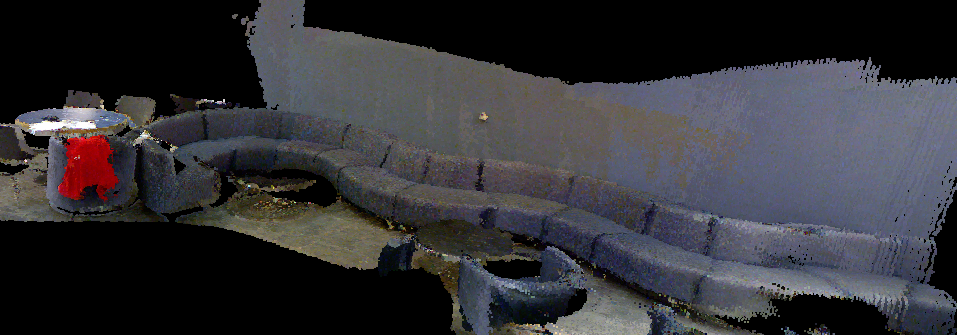
\includegraphics[width=0.9\textwidth]{figures/awesome_couch.png}
\caption{A reconstruction of the couches in Tishman Hall.}
\label{fig:couch}
\end{figure*}

\subsubsection{Computing the Rigid Body Transformation}
After features are extracted using SURF from the RGB images, we project
them into 3D space using the depth data from the Kinect. Given these
corrseponding 3D features, we may estimate the movement of the camera
between the frames using Horn's algorithm and RANSAC.

Horn's algorithm is a closed-form calculation of the optimal rigid body
transformation in three or more dimensions.  Given a set of corresponding
points it calculates the optimal transformation without iteration
~\cite{horn1987closed}.  The majority of the calculations we perform with
Horn's algorithm have only three sets of corresponding 3D points, and so
Horn's algorithm is quite fast.

Horn's algorithm is used at every iteration within our RANSAC implementation.
We use RANSAC to discover outliers in the set of corresponding features
set. At each iteration of RANSAC, three corresponding pairs of features
are selected randomly; this is the minimum needed to model a rigid body
transformation. The optimal alignment between these pairs is computed using
Horn's algorithm. The consensus voting is based on the reprojection error.
For every potential correspondence between 3D points $A_i$ and $B_i$,
the rigid body transformation $T$ receives a ``yes'' vote if
$\parallel A_i - TB_i \parallel < K$. In our implementation, $K$ is 10\,cm.

RANSAC halts after a given number of iterations or after $80\%$ of the
correspondences are considered to be inliers.  This was done to decrease
the time spent in RANSAC, however in practice, inlier sets rarely exceeded
$80\%$ of the total number of corresponding features.  An initial
transformation is then computed using just the optimal inlier set.

We have experimented with using adaptative RANSAC, as described in~\cite{Hartley2004}.
The goal of this algorithm is to estimate the ratio of inliers, and therefore the number
of iterations needed to arrive at a solution that has only inliers with a level $p$ of
confidence. Adaptative RANSAC starts by presuming a worst case scenario where
there are no inliers, and therefore infinite iterations would be needed. This estimate is
then refined at every iteration. If the number of consensus votes that a rigid-body
transformation gets is greater than the current estimate of the number of inliers,
that estimate is refined, along with the number of iterations needed.

As expected, using adaptative RANSAC decreased the average number of iterations significantly.
However, our experiments showed that the quality of the resulting transformations was worse
than when using normal RANSAC. Additionaly, the number of inliers detected was also smaller.
We believe that these issues could be ironed out, but we did not give it much further attention
due to time constraints, and the fact that plain RANSAC was giving good enough results
for our purposes.

\subsection{ICP}
	The rigid body transformation (RBT) calculated by aligning corresponding visual features can be further refined by aligning point clouds between successive frames.  Iterative Closest Point (ICP) is one method to accomplish this.  ICP is an iterative processes that alternates between using a given rigid body transformation to determine point correspondences and using these point correspondences to compute an RBT to align the points.  \newline

\begin{algorithm}
\begin{algorithmic}
\REQUIRE pointclouds $A = a_{i}$, $B = b_{i} $, initial transformation $T_{0}$
\STATE $T = T_{0}$
\WHILE {\emph{not converged}}
\FOR {$i = 1 \to N$}
\STATE $a^{B}_{i} \in B = T * a_i$
\STATE $n_{i} =$ nearested point in $B(a^{B}_{i})$
\ENDFOR
\STATE $T = argmin_{T} \{\sum_{i} ||T * a_{i} - n_{i} ||^2\}$
\ENDWHILE
\end{algorithmic}
\end{algorithm}

	Let point cloud A be the point cloud corresponding to the most recent frame received from the Kinect and let point cloud B be the previous one received.  ICP applies an initial estimate of the RBT between $A$ and $B$, to the each of the points, $a_{i}$ in $A$ to get points a in frame $B$.  Simple nearest neighbor data association determines point correspondences which is accelerated through the use of a K-D tree.  Then using Horn's algorithm we compute the optimal RBT to align the corresponding points~\cite{horn1987closed}.  We made use of the AlignPoints3D April code for this computation.  Then we compute the error in the alignment by taking the sum of the distances between corresponding points.  This whole process is repeated until the decrease in error from one iteration to the next has increased above a set threshold.

	Unfortunately, simple ICP as described above has quite a few weaknesses, some of which we have attempted to address
by emulating the methods described in A. Segal's Generalized ICP~\cite{gicp}.

	ICP uses a point to point error metric which implicitly assumes that our sensor has measured the same point from both frames.  However this is not a completely rigorous or robust way of describing how two views of a scene are related to one another, since it is exceedingly unlikely that our sensor will sample the exact point in each view.  Alternative formulations of ICP, such as Iterative Closest Plane, which minimizes a point to plane error metric deal with this problem to some degree.  Iterative Closest Plane introduces the additional complication of computing normal vectors for each point in one of the views.  This more complicated formulation would yield improved accuracy, however there are other areas where we could improve the project that would provide greater benefits for less cost in development time, so we avoided utilizing this more difficult formulation.

	ICP's nearest neighbor data association also implicitly assumes that the two point clouds being matched completely overlap.  In the vast majority of cases, movement of the sensor means that there will be points in one point cloud that do not correspond to points in the other point cloud.  Inaccurate point correspondences lead to distortions in the RBT.  The absence of corresponding point in the other view can occur for points that are near occlusion boundaries or close to the maximum range of the sensor.  It would be possible to construct a heuristic that would reason about occlusions and sensor range to avoid matching such points.  As a substitute for this more complex reasoning we introduce a horizon for point correspondences which limits the maximum distance between corresponding points.   If the nearest neighbor if beyond this horizon, then the correspondence is discarded.  However, this horizon introduces other complications.  If it is set to be too short, then the initial alignment will need to be very good to make any correspondences at all.  On the other hand if it is too long, then there will be no effect on the correspondences that are made.  In practice the alignment that RANSAC provides is good enough  to set a short horizon which all but eliminates this problem.

	There is still one, more troubling issue that a data association horizon introduces.  If the algorithm uses an error metric that is simply the sum of the distances between corresponding points, then it is plausible for the error to increase as the alignment improves if this horizon is used.  Given two point clouds and an initial alignment that puts most of the points beyond the horizon for data association.  The initial error will be relatively small because only a small number of correspondences will exist between the two clouds.  As the alignment is improved, more point correspondences will be discovered, which would cause the total error to increase.  This could cause the algorithm to terminate prematurely, leading to suboptimal alignments.  To solve this issue we use a normalized error metric which is simply the average error per correspondence.  Using this metric, the error will decrease correctly as the alignment is improved.

	ICP also requires a good initial alignment in order to guarantee that it converges to the global minimum error.  If we have a poor initialization, ICP will get caught in a local minimum.  Using visual feature correspondences provides a good enough estimate of the RBT that this problem is completely taken care of.

	Another major issue with ICP and other scan matching schemes like multi-resolution scan matching is that some scene geometries can make motions ambiguous.  For example moving down the length of a hallway would yield no change in the 3D range scans read by the Kinect or other similar sensors making it impossible to tell that the sensor has moved at all.  In fact, ICP would converge to a solution that would claim that the sensor has not moved at all, since such a solution would yield the greatest overlap of the two point clouds.  If such an environment has visual features, we can use these features to augment the alignment algorithm, as originally described in Henry's paper~\cite{Henry2010RGBd}.  This modification, described below, yields significantly improvements even in cases where there were no ambiguities in the environment.

\subsection{RGBD-ICP}
Using visual features to augment point cloud matching improves the quality of alignments produced by this step.    To utilize visual features we introduce the 3D coordinates relative to the Kinect, of inlier feature correspondences, into both point clouds.  Since their correspondence has already been determined by matching SURF descriptors and then filtered with RANSAC, these correspondences remain constant throughout each iteration of ICP.

\begin{algorithm}
\begin{algorithmic}
\REQUIRE pointclouds $A = a_{i}, B = b_{i}$, initial transformation $T_{0}$, corresponding visual features $Fa_{i}, Fb_{i}$
\STATE $T = T_{0}$
\WHILE {\emph{not converged}}
\FOR {$i = 1 \to N$}
\STATE $a^{B}_{i} \in B = T * a_i$
\STATE $n_{i} = $ nearest point in $B(a^{B}_{i})$
\IF {$||n_{i}-a^{B}_{i}|| \leq d_{threshold}$}
    \STATE $w_i = 1$
\ELSE
    \STATE $w_i = 0$
\ENDIF
\ENDFOR
\STATE $T = argmin_{T} \{\sum_{i} w_{i}||T*a{i} - n_{i} ||^2 + m_{i} ||T*Fa_{i} - Fb_{i}||^2\} $
\ENDWHILE
\end{algorithmic}
\end{algorithm}

	Visual features are generally out-numbered by other points in the point cloud, so we have introduced a correspondence weighting term and modified the AlignPoints3D class to utilize this weight when computing the optimal transformation.  By increasing the weight of visual features relative to other points in the point cloud we can ensure that they influence the alignment to the degree that we want.  To achieve a relative weight of 50\% where as a whole both the point cloud and the visual features have approximately same say in the final alignment, each visual feature correspondence is given a weight, $m_{i}$, equal to the size of the point cloud divided by the number of feature correspondences.  It would be more accurate to calculate the number of point correspondences and use that rather than the size of the point cloud.  Conceptually this weighting procedure is equivalent to duplicating each of the visual features to increase their influence on the alignment.  However this formulation for the weight becomes problematic at low inlier correspondence numbers as increasingly few features are given greater and greater weight when in fact we should trust visual features less if there are so few to use in the first place.  To address this issue, the maximum weight assigned to each visual feature is capped at a maximum number ensuring that the influence of the point cloud grows as visual features become less reliable.

\subsection{Constant Velocity Motion Model}
In circumstances when there are few or no visual features, we would still like to estimate the RBT between frames to initialize ICP.  As in the paper, we implemented a constant velocity model which uses the RBT estimated by RGBD-ICP at each time step combined with a timer to estimate the linear and angular velocities of the Kinect.  These values averaged over time to attempt to reduce the noise that velocity estimates are prone to, however this tends to introduce time delays in the response of the estimated velocity compared to the actual velocity of the Kinect.  We found that once the set of inliers features from RANSAC dropped to about 20, it would no longer give accurate RBTs.  At this threshold, the constant velocity motion model steps in and provides an estimate to initialize ICP.

By definition the constant velocity model assumes that the Kinect maintains a constant velocity so large changes in the motion of the sensor in areas without visual features causes the system to fail.  Additionally there are cases where both a lack of visual features and the presence of a geometric ambiguiity cause both RANSAC and RGBD-ICP to fail.  This simultaneous failure quickly renders the constant velocity model useless since its estimates are quickly ruined by the erroneous results from RGBD-ICP.  We attempted to deal with this problem by setting internal limits on how rapidly the estimates of velocity could change, but our implementation currently has no heuristics to determine when RGBD-ICP has failed leading to poor behavior in circumstances when the constant velocity model alone might yield better results.  Improvements in this area would greatly increase the reliability of the system in many common situations such as mapping large empty sections of large rooms, where features are beyond the range of the sensor or if the sensor is looking at a featureless wall for brief periods of time.



\subsection{Rendering the Scene}
We do not attempt to implement the surfels demonstrated by Henry et al.
Surfels, while excellent at preserving detail, are a huge engineering
undertaking in and of themselves, and it is extremely costly to
update their values during data collection. Surfels alone would destroy our
chances of rendering updates to the scene in real time. Instead, we chose to
store data as voxels of a fixed resolution. Voxel updates, while not free, are
incredibly cheap in comparison to surfel updates and
individual voxels do not change in memory requirements over time. Our
voxels store a running total of the ARGB values observed in that bin and are
treated as being colored as an average of these observations.

Henry et al. wrote a custom tool to allow them to navigate surfel environments
in real time~\cite{Henry2010RGBd}. Again, this was a large engineering effort
and was not our main priority. Instead, we render all of our voxels at once,
as cubes, regardless of on screen visibility. The performance for this
rendering scheme proved to be unacceptable, so our voxels are instead rendered
as individual points rendered at the center of their respective bins. As a
result, scenes are best viewed from some distance so as to mask the gaps
between the points. To facilitate 3D navigation through the scene, we employ a
Logitech gamepad supporting translation in the current camera plane as well as
in place rotation of the camera.

\section{Evaluation}
\begin{figure}[t]
\centering
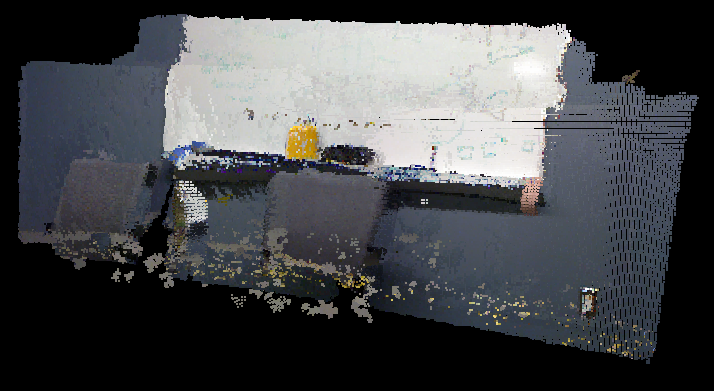
\includegraphics[width=0.48\textwidth]{figures/cropped_gt_slc.png}
\caption{The reconstruction of one of the whiteboards in the student learning center,
in the CSE building. This dataset was used to evaluate the system.}
\label{fig:gt-slc}
\end{figure}

\subsection{Ground Truth Evaluation}
The end goal of our system is to provide rich 3D reconstructions of indoor environments.
It is hard to quantify the quality of those reconstructions, and therefore to numerically
judge the performance of the system. However, we can estimate the error in the visual odometry,
which is the most important factor in the reconstruction of the environment. This provides
a decent approximation of the quality of the final output.

Our first try at an experiment involved using AprilTags~\cite{olson2011tags} to
provide ground-truth localization. Because the size of the tags are known, it is
possible to know their 3D positions relative to the camera. If we assume that the tags are fixed and that
the detection of the tags is precise enough, we can use the movement of the
Kinect in relation to the tags as the ground-truth. However, we have found that
the RGB images were not of sufficient quality to provide accurate and consistent
detection of the tags. In particular, debayering artifacts were clearly noticable.
This is problematic because the tags are black and white. The debayering blurs the
image around the edges in such a way that the detected position of the tags is very noisy.

We therefore resorted to a simple ground-truth experiment. Instead of measuring the actual trajectory of
the Kinect, we physically marked a number of checkpoints on the world,
and moved the Kinect from one to the other. At every one of those checkpoints, we recorded the
Kinect's estimated position, with the first checkpoint being at the origin. At the end of the
test run, we compared the Kinect's esimate of the checkpoints to where they really were in the
world.

\begin{figure}[t]
\centering
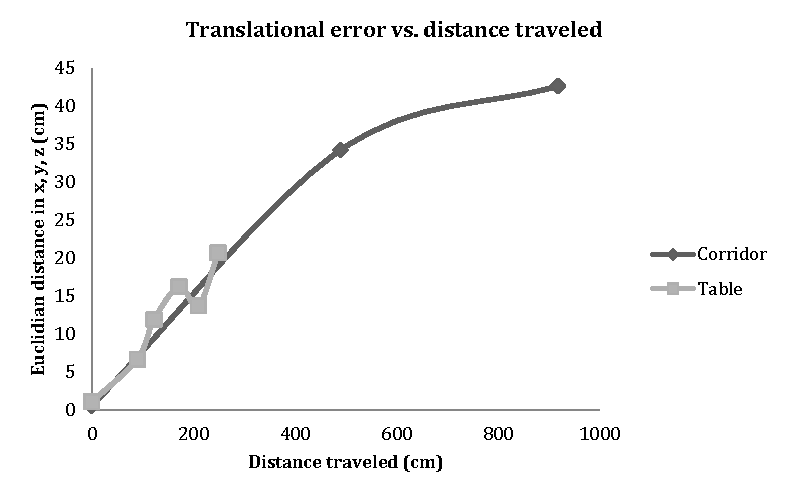
\includegraphics[width=0.48\textwidth]{figures/gt_translational.pdf}
\caption{The errors in the x, y and z coordinates as the Kinect moves between the checkpoints
for the two datasets.}
\label{fig:plot-trans}
\end{figure}

We performed this evaluation in two environments. Fig.~\ref{fig:cse-wall} shows the reconstruction of a
feature-rich hallway. Three checkpoints were placed on the ground along the hallway, and the Kinect was
moved between them. Fig.~\ref{fig:gt-slc} is the reconstructed whiteboard in the student learning
center in CSE. For this test, six checkpoints were placed in a zig-zag pattern on a table.

Fig.~\ref{fig:plot-trans} shows the translational error at every checkpoint for both datasets.
As expected from a pure odometry system, the error acumulates and the estimative of the Kinect's
position tends to diverge with time. Fig.~\ref{fig:plot-angular} presents the angular error at
every checkpoint. The ``table" dataset shows significantly greater errors because of the
zig-zag pattern of the markers, which caused angular errors to accumulate more rapidly.

We also conducted a number of reconstructions without ground-truth data. Fig.~\ref{fig:couch}
is an example of a reasonably long trajectory for which our system produced a good
reconstruction.

\subsection{Real-time Performance}
Given our simplification of the original problem (namely not implementing SLAM
or surfels), one of our major goals was to be able to collect and add data to
our global point cloud in real-time. By switching from SIFT to SURF, for
example, we reduced the cost of processing a frame for features from
~180\,ms per frame to ~9\,ms per frame. The total cost of processing a frame
for a variety of voxel resolutions
can be seen Table~\ref{tbl:match-times}. Generating voxels clearly dominates the
processing time, taking 78\% of the total time for 1\,cm of resolution
(generally the smallest resolution we operate at). Still, this is as opposed
to surfel updates in Henry et al.'s work, which were reported to take roughly
6 seconds per frame, so we still consider this a vast improvement. Though by
no means fast enough to keep up with the full speed of the Kinect, this allows
us to update scenes at between 7-20\,fps depending on our needs.

\begin{table}
    \centering
    \begin{tabular}{ | c || r | r | r | }
    \hline
    Resolution & 1\,cm  & 2\,cm & 4\,cm \\
    \hline
    \hline
    SURF & 9\,ms &9\,ms & 9\,ms \\
    \hline
    RANSAC & 16\,ms & 16\,ms & 16\,ms\\
    \hline
    ICP & 5\,ms & 5\,ms & 5\,ms \\
    \hline
    Voxelization & 105\,ms & 47\,ms & 21\,ms \\
    \hline
    {\bf Total} & {\bf 135\,ms} & {\bf 77\,ms} & {\bf 51\,ms} \\
    \hline
    \end{tabular}
\caption{Time spent at each stage of point cloud processing for varying voxel
    resolutions. As expected, voxels are still extremely costly to process,
    but small reductions in voxel resolution lead to dramatically improved
    results.}
\label{tbl:match-times}
\end{table}

Real time rendering performance is another issue. Though we are able to
process the data quickly enough and add it to our global point cloud in
real-time, rendering the frame is incredibly costly, especially as the global
point cloud grows. A 30 second dataset collected of a medium sized office
contains over 2 million voxel points at 1\,cm resolution, and visual
updates/real-time navigation of this scene lag noticeably behind input. Our
experience shows that the system delivers real-time visual updates and
navigability when running with 2\,cm voxels. For live demonstrations, this is
the resolution we employ. Rendering times obviously increase with the number
of points in the scene, as we do nothing to stop rendering points we cannot
see. However, even after only several seconds of data collection, rendering
the scene at 1\,cm resolution takes over half a second whereas a similar scene
at 2\,cm or 4\,cm resolution takes between 200-250\,ms. This means that,
despite our ability to process data faster than this, updates to the scene
appear slowly from the viewer's perspective. We believe that 4-5\,fps falls
clearly into the realm of real-time, though, and found this performance
adequate for demonstration purposes.

\section{Conclusion}
We successfully implemented a simplified version of Henry et al.'s RGB-D mapping
system that is able to make 3D reconstructions of the surrounding environment
using a Kinect sensor~\cite{Henry2010RGBd}. Modifications to the original
design allow our system to run in real time, though we are unable to keep up with
the full speed of our sensor, forcing us to throw away some data. The addition of
visual features to depth information allow us to accurately maintain our position
estimate in the world even in environments lacking unique depth data. Though our
system could clearly benefit from the addition of a full SLAM system to
correct our slowly accumulating error, as exemplified in Fig.~\ref{fig:slam},
 we are still able to maintain position
estimates within a 10\% error margin of the total distance traveled.

\begin{figure}[t]
\centering
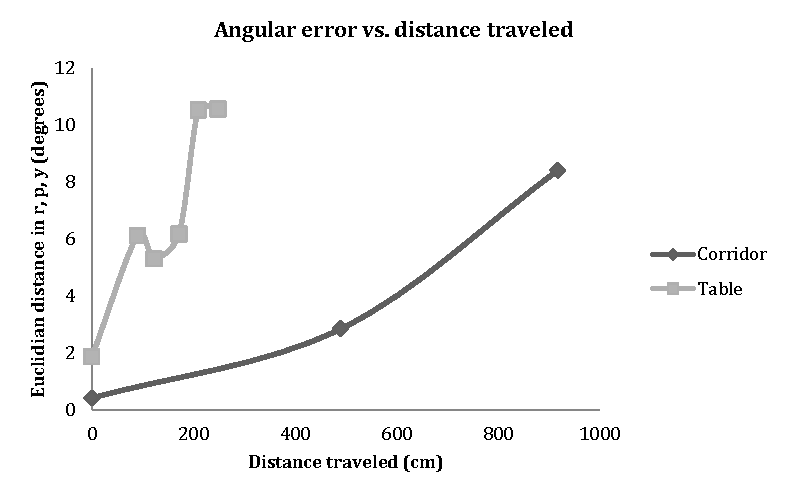
\includegraphics[width=0.48\textwidth]{figures/gt_angular.pdf}
\caption{The errors in roll, pitch and yaw as the Kinect moves between the checkpoints
for the two datasets.}
\label{fig:plot-angular}
\end{figure}

\section*{Acknowledgements}
This was also the final project for EECS 568. Lauren Hinkle and Robert Goeddel
contributed extensively to the development of the system
and also to the EECS 568 report, which served as basis for this document. However,
the majority of this report was written by the three authors. In particular, the
section on Methodology was written almost entirely by the authors.

Special thanks to Pradeep Ranganathan for providing some extra depth
information in Fig.~\ref{fig:Kinect-demo} and Prof. Ed Olson for patiently
posing for us in Fig.~\ref{fig:ed-model}.

% XXX References
\bibliographystyle{IEEEtranS}
\bibliography{sources}


\begin{figure}[t]
\centering
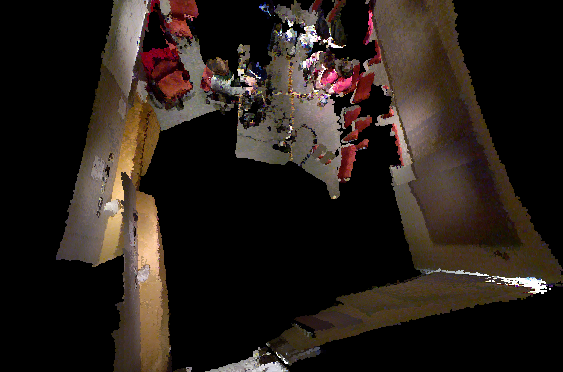
\includegraphics[width=0.48\textwidth]{figures/slam.png}
\caption{An example of a dataset that would have greatly benefitted from loop-closures.}
\label{fig:slam}
\end{figure}

\end{document}